\documentclass[11pt]{article}

% ---------------------------------------------------------------------------
% World-Model-Based RL for Robotic Manipulation:
% A study of World4RL and WoVR, and a from-scratch reliability reproduction.
% Compile with:  pdflatex world_model_rl_study.tex   (run twice for refs)
% Place at the repository root so the \includegraphics paths resolve; each
% figure is guarded with \IfFileExists so the document compiles even if the
% PNGs are absent.
% ---------------------------------------------------------------------------

\usepackage[utf8]{inputenc}
\usepackage[T1]{fontenc}
\usepackage[margin=1in]{geometry}
\usepackage{amsmath,amssymb}
\usepackage{booktabs}
\usepackage{graphicx}
\usepackage{caption}
\usepackage{enumitem}
\usepackage{xcolor}
\usepackage[colorlinks=true,linkcolor=blue,citecolor=blue,urlcolor=blue]{hyperref}

\newcommand{\Egap}{\ensuremath{\mathrm{Gap}}}
\newcommand{\Jmodel}{\ensuremath{J_{\mathrm{model}}}}
\newcommand{\Jreal}{\ensuremath{J_{\mathrm{real}}}}

\title{\textbf{World-Model-Based Reinforcement Learning for Robotic Manipulation}\\[4pt]
\large A Technical Study of \textsc{World4RL} and \textsc{WoVR},\\
and a From-Scratch Reproduction of Their Reliability Mechanisms}
\author{Jiaqi Tang\\ \small University of Illinois Urbana-Champaign\\ \small \texttt{github.com/TanhJK728/world-model-rl}}
\date{\today}

\begin{document}
\maketitle

\begin{abstract}
Learned world models promise to replace costly and unsafe real-robot interaction with policy
optimization performed entirely ``in imagination.'' The central research question has shifted from
\emph{whether} a generative model can imitate real dynamics to \emph{how} reinforcement learning (RL)
can stay reliable when those dynamics are imperfect --- under hallucination, long-horizon error
accumulation, and policy-induced distribution shift. This report first gives a detailed technical
account of two works from Chao Yu's group along this trajectory: \textsc{World4RL}, which establishes
diffusion world models as high-fidelity simulators for refining pre-trained manipulation policies,
and \textsc{WoVR}, which treats reliability as the first-class problem and regulates the RL--model
interface for post-training Vision--Language--Action (VLA) policies. We then present a compact,
from-scratch reproduction (continuous-control PPO, a bootstrapped dynamics ensemble, and
uncertainty-aware imagined refinement) that isolates the same mechanisms on a controllable
\texttt{Pendulum-v1} toy and independently rediscovers two of their central premises: reliable
imagined refinement depends on the world model's \emph{coverage} of the policy's state distribution,
and uncertainty signals must be \emph{recalibrated} as the policy drifts.
\end{abstract}

\tableofcontents
\bigskip

% ===========================================================================
\section{Motivation and the research question}
% ===========================================================================
Robotic manipulation policies are typically bootstrapped by imitation learning (IL), whose ceiling is
set by the scarcity and narrow coverage of expert data. RL can refine such policies, but on-policy RL
needs massive interaction: real-robot training is costly and unsafe, and physics simulators incur a
sim-to-real gap. Generative world models offer a third path --- a \emph{learned} simulator in which a
policy can be improved without touching the real world.

The difficulty is that a learned world model is not a faithful simulator. In closed-loop, autoregressive
rollouts, small one-step errors compound with the horizon, and as the policy improves its state--action
distribution drifts away from the model's training data. If RL naively trusts these rollouts, it is
incentivized to \emph{exploit systematic model errors} rather than make real task progress: a policy can
look excellent in imagination and fail in reality. Both papers below take this as the core problem; our
reproduction measures it directly.

% ===========================================================================
\section{World4RL: Diffusion World Models for Policy Refinement}
% ===========================================================================
\textbf{Jiang et al., ``World4RL: Diffusion World Models for Policy Refinement with Reinforcement
Learning for Robotic Manipulation'' (2025).}

\subsection{Idea}
World4RL is a two-stage framework: (i) \emph{pre-train} a diffusion world model on multi-task data to
capture diverse dynamics, then (ii) \emph{freeze} it and refine an IL-initialized policy entirely inside
it with PPO, avoiding online real-world interaction. Unlike prior work that uses generative models for
test-time \emph{planning} (e.g.\ IRASim, NWM) or RSSM-based latent models that produce blurry, drifting
rollouts (DiWA), World4RL uses a sharp diffusion backbone to support end-to-end policy optimization.

\subsection{Method}
The framework has three learned components: a \textbf{diffusion transition model} $D_\theta$
(dynamics), a \textbf{reward classifier} $C_\psi$ (sparse binary success signal), and the
\textbf{policy} $\pi_\xi$ (refined with PPO).

\paragraph{Stage 1 --- pre-training.}
\begin{itemize}[leftmargin=1.4em,itemsep=2pt]
  \item \emph{Policy}: a Gaussian policy $\pi_\xi(a_t\mid x_t)=\mathcal{N}(\mu_\xi(x_t),\Sigma_\xi(x_t))$
  trained by behavior cloning, $\mathcal{L}_{\mathrm{BC}}(\xi)=-\mathbb{E}_{(x_t,a_t)\sim\mathcal{D}_{\exp}}[\log\pi_\xi(a_t\mid x_t)]$.
  \item \emph{Reward classifier}: $r:=C_\psi(x_{t+1})$, a ResNet-18 trained with binary cross-entropy on
  both expert data and pre-trained-policy rollouts, so it recognizes success states the learned policy
  actually reaches.
  \item \emph{Diffusion transition model}: following EDM, a preconditioned denoiser
  $D_\theta(x_\tau;\tau,c)=c^\tau_{\mathrm{skip}}x_\tau+c^\tau_{\mathrm{out}}F_\theta(c^\tau_{\mathrm{in}}x_\tau;c^\tau_{\mathrm{noise}},c)$
  predicts the next observation from a short history $x_{t-T:t}$ and actions. A key design is the
  \textbf{two-hot action encoding} (from DreamerV3): each continuous action dimension $a_i$ is mapped
  onto its two nearest bins $b_k\le a_i\le b_{k+1}$ with weights
  $t_i[k]=\tfrac{b_{k+1}-a_i}{b_{k+1}-b_k},\; t_i[k{+}1]=\tfrac{a_i-b_k}{b_{k+1}-b_k}$,
  a lossless, differentiable representation ($K\!\approx\!21$ bins) that avoids the reconstruction errors
  of tokenization or latent compression. Crucially, $D_\theta$ is trained on a \emph{mixture}:
  expert demonstrations $\mathcal{D}_{\exp}$, pre-trained-policy rollouts $\mathcal{D}_{\mathrm{rollout}}$,
  and \emph{uniformly random} rollouts $\mathcal{D}_{\mathrm{rand}}$, so the model sees a broad range of
  transitions and does not overfit the narrow expert set.
\end{itemize}

\paragraph{Stage 2 --- policy optimization.}
The frozen $D_\theta$ generates imagined rollouts; $C_\psi$ scores each imagined next state as a sparse
binary reward; $\pi_\xi$ is updated with the clipped PPO objective
\begin{equation}
\mathcal{L}_P(\xi)=\mathbb{E}_t\!\left[\min\!\big(\rho_t(\xi)A_t,\;\mathrm{clip}(\rho_t(\xi),1-\epsilon,1+\epsilon)A_t\big)\right],
\quad \rho_t(\xi)=\frac{\pi_\xi(a_t\mid x_t)}{\pi_{\xi_{\mathrm{old}}}(a_t\mid x_t)},
\end{equation}
with a squared-error value loss. Because optimizing inside the model tends to push the policy toward
out-of-distribution (OOD) actions where the model is unreliable, World4RL adds \textbf{controlled
exploration}: the policy standard deviation is clipped to a conservative bound $\sigma\le e^{0}$ (versus
the common $\sigma\le e^{2}$), keeping sampled actions near the support of the model's training data.

\subsection{Experiments}
\paragraph{World-model fidelity (Meta-World video prediction).} With 330M parameters, World4RL attains
the best FVD/FID/LPIPS among NWM, iVideoGPT, and DiWA under both policy and random rollouts
(Table~\ref{tab:w4rl-vp}), and faithfully models even \emph{failure} trajectories where baselines
hallucinate success.

\begin{table}[h]
\centering
\caption{World4RL video-prediction fidelity on Meta-World (lower is better).}
\label{tab:w4rl-vp}
\begin{tabular}{lcccccc}
\toprule
 & \multicolumn{2}{c}{FVD} & \multicolumn{2}{c}{FID} & \multicolumn{2}{c}{LPIPS}\\
\cmidrule(lr){2-3}\cmidrule(lr){4-5}\cmidrule(lr){6-7}
Model & Policy & Random & Policy & Random & Policy & Random\\
\midrule
\textbf{World4RL} & \textbf{326.5} & \textbf{400.1} & \textbf{17.1} & \textbf{23.4} & \textbf{0.019} & \textbf{0.025}\\
NWM       & 547.4 & 851.9 & 30.5 & 34.9 & 0.027 & 0.026\\
iVideoGPT & 450.3 & 531.3 & 18.7 & 20.7 & 0.026 & 0.028\\
DiWA      & 803.6 & 1231.0 & 62.9 & 96.5 & 0.080 & 0.136\\
\bottomrule
\end{tabular}
\end{table}

\paragraph{Policy learning (Meta-World, sparse reward, 6 tasks, 3 seeds).} World4RL reaches the best
average success rate $67.5\%$, a $+16$-point absolute gain over the BC base ($51.5\%$), beating IL
(BC, Diffusion Policy), offline RL (TD3+BC, IQL), and world-model baselines (IRASim, DiWA, TD-MPC2).
It matches offline-to-online methods (RLPD, Uni-O4) while using \emph{no} online samples, versus their
$346$k/$470$k online steps.

\paragraph{Real robot (Franka Panda, 6 tasks, 20 trials each).} World4RL reaches $93.3\%$ average
success, a $+25$-point gain over BC ($68.3\%$) and above Diffusion Policy ($88.3\%$), and executes
tasks more decisively.

\paragraph{Ablations.} (i) Two-hot encoding beats linear/one-hot/VQ-VAE/tokenization on all fidelity
metrics. (ii) Removing \emph{action-std clipping} or \emph{random rollouts} both degrade policy
performance and increase variance --- validating that \textbf{controlled exploration} and \textbf{broad
action-space coverage} are critical to stable imagined refinement.

\subsection{Conclusions}
Diffusion world models can serve as high-fidelity, real-time simulators enabling consistent
PPO refinement of pre-trained policies under sparse rewards, without online interaction. The authors
explicitly flag the open direction of ``more robust RL algorithms that can effectively learn under
imperfect learned dynamics.''

% ===========================================================================
\section{WoVR: World Models as Reliable Simulators for Post-Training VLA Policies}
% ===========================================================================
\textbf{Jiang, Zhou et al., ``WoVR: World Models as Reliable Simulators for Post-Training VLA Policies
with RL'' (2026).}

\subsection{Idea}
WoVR reframes world-model-based RL as a \emph{reliability} problem rather than a modeling problem.
It defines \textbf{hallucination} as a systematic mismatch between imagined and real outcomes in
closed-loop interaction, driven by two compounding effects: \emph{autoregressive feedback} (the model
conditions on its own generated frames, amplifying early errors) and \emph{distribution shift} (the
evolving policy drifts from the world model's training data). WoVR controls hallucination at three
interconnected levels rather than assuming a faithful simulator.

\subsection{Method}
\paragraph{(1) Stabilized action-conditioned world model.} Built on the Wan2.2-TI2V-5B video-diffusion
backbone and reformulated as an action-conditioned generator. Actions are injected through a
\textbf{dual-channel} design (timestep-conditioned normalization plus replacing text embeddings in
cross-attention), giving frame-level control while preserving the DiT structure. A
\textbf{first-frame--anchored} context $[o_0,\,o_{t-c:t}]$ fixes global layout while memory frames
preserve local dynamics, and \textbf{noisy context augmentation} corrupts non-reference context frames
during training so the model is robust to its own generated frames at inference. It is trained with a
rectified-flow objective $\mathcal{L}=\mathbb{E}\,\lVert u(x_\tau,c,\tau;\phi)-(x_1-x_0)\rVert^2$ with
$x_\tau=(1-\tau)x_0+\tau x_1$. Reward is supplied by either a lightweight ResNet (sparse binary) or a
Qwen3-VL model (dense ordinal progress $\ell_t\in\{0,\dots,10\}$).

\paragraph{(2) Keyframe-Initialized Rollouts (KIR).} Instead of always starting imagined rollouts from
the episode start $o_0$ --- which forces the model to imagine a long, drift-prone prefix before reaching
decisive contacts --- KIR initializes a portion of rollouts from \emph{keyframes} $o_k$ near
task-critical (often failure) states, using $[o_0,\,o_{T_{\mathrm{KIR}}-3:T_{\mathrm{KIR}}}]$ as context.
This \emph{shortens the effective prediction depth}, reducing hallucination compounding. The policy is
updated with GRPO,
\begin{equation}
\mathcal{J}_{\mathrm{GRPO}}(\theta)=\mathbb{E}\!\left[\frac{1}{G}\sum_{i=1}^{G}\frac{1}{T^{\mathrm{valid}}_i}\sum_{t=1}^{T^{\mathrm{valid}}_i}\min\!\big(\rho^{(i)}_t(\theta)\hat A^{(i)},\,\mathrm{clip}(\rho^{(i)}_t(\theta),1-\epsilon,1+\epsilon)\hat A^{(i)}\big)\right],
\end{equation}
where $\hat A^{(i)}$ is a group-relative advantage and $T^{\mathrm{valid}}_i$ counts steps up to first
success; trajectory-length normalization lets short, task-critical (KIR) segments dominate the gradient
over long drift-prone continuations.

\paragraph{(3) PACE: policy-aligned co-evolution.} Because policy optimization shifts the action
distribution away from the world model's training data, WoVR periodically re-aligns them: train an
initial $\mathrm{WM}_{\mathrm{Base}}$ on base-policy trajectories, optimize the policy inside it, then
collect a \emph{small} set of rollouts under the evolved policy to refine the model into
$\mathrm{WM}_{\mathrm{Evo}}$. This is \emph{low-frequency} (unlike classical MBRL's high-frequency model
updates), so it needs no continuous supervision while restoring simulator reliability.

\subsection{Experiments}
\paragraph{World-model quality (LIBERO, 512-frame closed-loop rollouts).} WoVR outperforms EVAC,
Cosmos-Predict2, and OpenSora on LPIPS/FID/FVD/FloLPIPS, with the margin \emph{growing} at longer
horizons, at $23$ FPS (vs OpenSora's $7$) despite a larger backbone --- via only five diffusion steps and
a 3D VAE.

\paragraph{Policy performance (LIBERO success rate).} Table~\ref{tab:wovr-sr} summarizes the headline
result under two SFT initializations. WoVR beats limited-budget online GRPO and the WMPO imagined-RL
baseline in every suite, with the largest gains where the base policy is weakest.

\begin{table}[h]
\centering
\caption{WoVR LIBERO success rates (\%). All methods share a 2{,}500-trajectory budget.}
\label{tab:wovr-sr}
\begin{tabular}{lccccc}
\toprule
Method & Spatial & Object & Goal & Long & Avg\\
\midrule
\multicolumn{6}{l}{\emph{One-trajectory SFT}}\\
OpenVLA-OFT (base) & 63.6 & 36.4 & 48.2 & 13.8 & 40.5\\
\;+ GRPO (online)  & 66.6 & 45.2 & 52.2 & 14.6 & 44.6\\
\;+ WMPO           & 67.8 & 65.4 & 56.6 & 13.8 & 50.9\\
\;+ \textbf{WoVR}  & \textbf{84.2} & \textbf{80.8} & \textbf{77.4} & \textbf{35.8} & \textbf{69.5}\\
\midrule
\multicolumn{6}{l}{\emph{Full-trajectory SFT}}\\
OpenVLA-OFT (base) & 93.6 & 83.0 & 90.0 & 85.6 & 88.1\\
\;+ WMPO           & 95.0 & 94.8 & 92.8 & 87.0 & 92.4\\
\;+ \textbf{WoVR}  & \textbf{98.8} & \textbf{98.8} & \textbf{94.8} & \textbf{91.4} & \textbf{96.0}\\
\bottomrule
\end{tabular}
\end{table}

\paragraph{Real robots.} On a Franka Panda, WoVR improves the base policy by $+28.9$ points (vs WMPO's
$+13.4$); on the noisier AgileX Piper by $+13.4$ (vs WMPO's $+3.4$), showing that naive imagined RL
remains vulnerable to hallucination while WoVR transfers reliably. The framework also generalizes to a
$\pi_{0.5}$ backbone ($+22.3$ points).

\subsection{Conclusions and limitations}
Hallucination in closed-loop imagined interaction is the central reliability bottleneck of
world-model-based RL for VLA; controlling it at the simulator, interaction, and alignment levels lets a
learned model act as a practical RL simulator. The authors note their analysis is empirical --- no formal
characterization of how hallucination propagates into policy optimization, and no regret bound of the
imagined-optimal policy relative to the real-optimal one --- and that longer-horizon and mobile
manipulation remain open.

% ===========================================================================
\section{This project: Reliable RL under Imperfect Learned Dynamics}
% ===========================================================================
\subsection{Positioning}
World4RL and WoVR operate at the frontier: diffusion/video world models, VLA policies, real robots. To
\emph{understand the mechanisms} rather than the engineering, this project builds the entire stack from
scratch in PyTorch on the controllable \texttt{Pendulum-v1} state space, where the exploitation gap can
be measured exactly. It is a state-space, dynamics-model MBRL study (in the lineage of PETS, MBPO, and
Dreamer's imagination step), not a generative video model; the transferable content is the
\emph{reliability mechanism}. The pipeline has four phases.

\subsection{Phase 1 --- Continuous-control PPO from scratch}
\texttt{Pendulum-v1} has observation $s_t=(\cos\theta_t,\sin\theta_t,\dot\theta_t)$, torque
$a_t\in[-2,2]$, and reward $r_t=-(\theta_t^2+0.1\,\dot\theta_t^2+0.001\,a_t^2)$. The policy is a
tanh-squashed Gaussian: sample $z\sim\mathcal{N}(\mu_\theta,\sigma_\theta^2)$ and set
$a=a_{\mathrm{scale}}\tanh(z)+a_{\mathrm{bias}}$, with the change-of-variables correction
\begin{equation}
\log\pi_\theta(a\mid s)=\log\mathcal{N}(z;\mu_\theta,\sigma_\theta^2)-\sum_i\log\!\big(a_{\mathrm{scale}}(1-\tanh^2 z_i)\big).
\end{equation}
Advantages use GAE-$\lambda$: with $\delta_t=r_t+\gamma V(s_{t+1})(1-d_{t+1})-V(s_t)$,
$\hat A_t=\sum_{l\ge0}(\gamma\lambda)^l\delta_{t+l}$, and the clipped PPO objective is optimized with a
clipped value loss and target-KL early stopping.

\paragraph{A reliability lesson already in Phase 1.} Out of the box the from-scratch PPO plateaus at
$\sim{-}1000$ (barely above random). The cause is scale: unnormalized Pendulum returns are $O(10^3)$, so
the critic loss is $\sim$2000--4000, giving noisy advantages. Adding \textbf{reward normalization} to the
training signal only (observations untouched, so the downstream world-model pipeline is unaffected) drops
the value loss to $\sim$0.05 and solves the task. Table~\ref{tab:ppo} reports the final policy.

\begin{table}[h]
\centering
\caption{Phase 1 deterministic evaluation (30 episodes). Config: $10^6$ steps, constant LR,
entropy coef.\ $0.01$, reward normalization.}
\label{tab:ppo}
\begin{tabular}{lc}
\toprule
Policy & Return (mean $\pm$ std)\\
\midrule
PPO seed 0 & $-148.7 \pm 94.4$\\
PPO seed 1 & $-152.7 \pm 100.9$\\
PPO seed 2 & $-157.5 \pm 100.5$\\
\textbf{Across seeds} & $\mathbf{-153.0 \pm 4.4}$\\
Random baseline & $-1198.6 \pm 280.7$\\
\bottomrule
\end{tabular}
\end{table}

\IfFileExists{../runs/ppo_summary/learning_curve_mean_std.png}{%
\begin{figure}[h]\centering
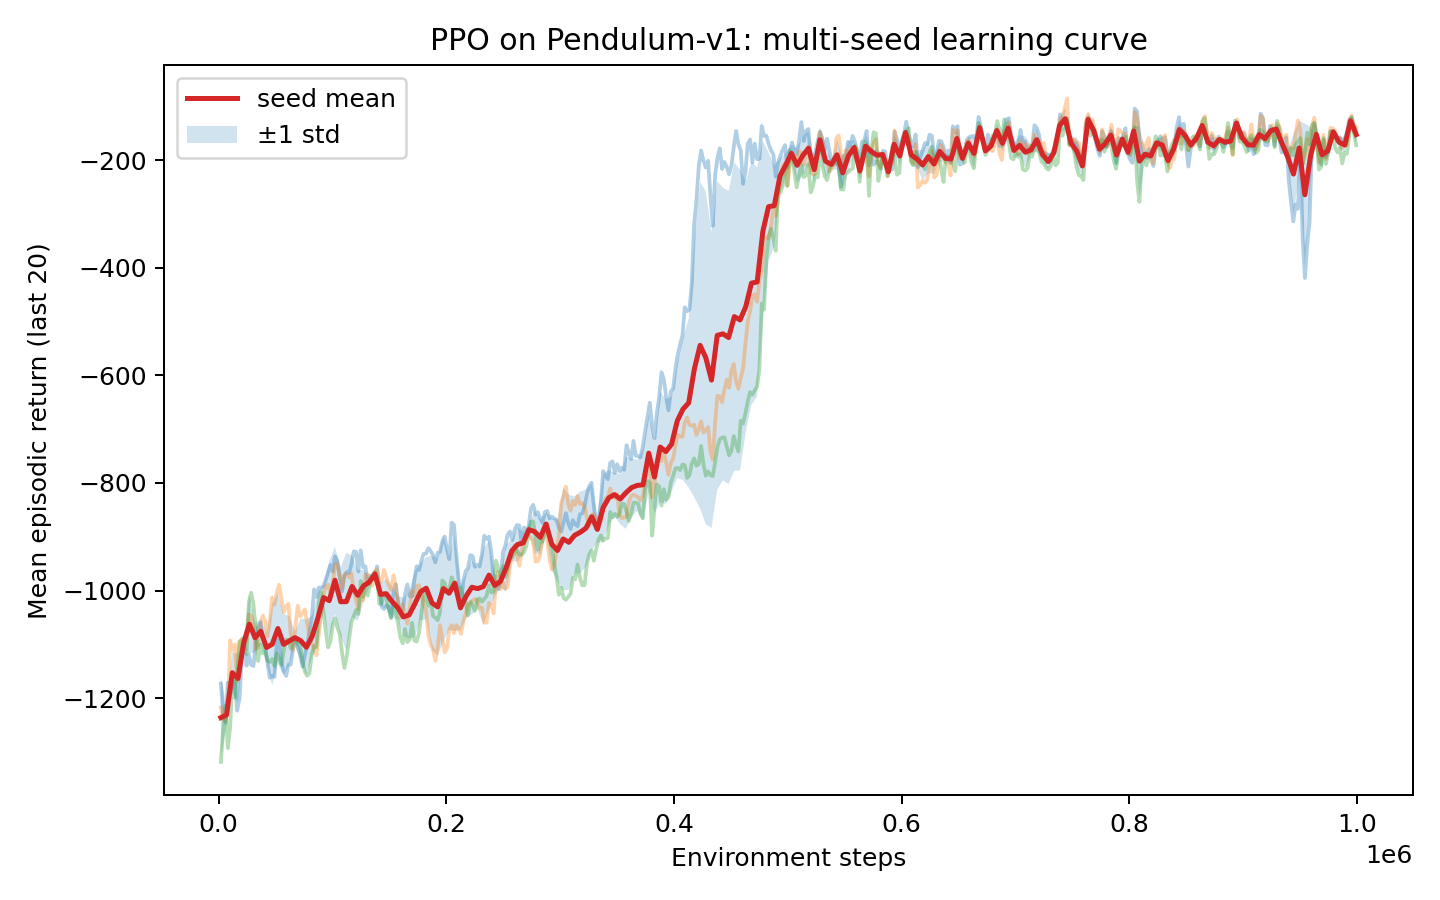
\includegraphics[width=0.72\linewidth]{../runs/ppo_summary/learning_curve_mean_std.png}
\caption{Multi-seed PPO learning curve: a sharp phase transition near 400--500k steps, then a stable
$\sim{-}150$ plateau.}
\end{figure}}{}

\subsection{Phase 2 --- Learned dynamics ensemble (the ``world model'')}
The world model is an ensemble of $K=5$ MLPs predicting the \emph{state delta},
\begin{equation}
\hat s_{t+1}^{(j)}=s_t+f_{\theta_j}(s_t,a_t),\qquad \Delta s_t=s_{t+1}-s_t,\quad j=1,\dots,K,
\end{equation}
with input/target normalization and a re-projection of $(\cos\theta,\sin\theta)$ onto the unit circle
after each step. Three deliberate choices mirror the papers' concerns: (i) \emph{no learned reward} ---
imagined rollouts use the exact Pendulum reward, isolating exploitation to dynamics error; (ii)
\emph{bootstrap ensemble + episode-level train/val split}; (iii) \emph{ensemble disagreement as epistemic
uncertainty},
\begin{equation}
u_t=\operatorname{mean}_k\operatorname{Var}_j\!\big[\hat s_{t+1,k}^{(j)}\big],
\end{equation}
calibrated into validation quantiles ($q_{95}=6.63\times10^{-6}$, the default rollout-termination
threshold).

\paragraph{Result: accurate on-distribution, unreliable off-distribution.} Trained only on
\emph{expert-policy} data, the model's error explodes under distribution shift
(Table~\ref{tab:wm-error}), and ensemble uncertainty rises in the same order --- a usable trust signal.
This is the toy-scale analogue of the hallucination that World4RL's random rollouts and WoVR's stabilized
model are designed to suppress.

\begin{table}[h]
\centering
\caption{Phase 2 world-model error by data source (model trained on \texttt{policy} only).}
\label{tab:wm-error}
\begin{tabular}{lccc}
\toprule
Source & one-step MSE & vs policy & mean uncertainty\\
\midrule
policy & $1.96\times10^{-6}$ & $1\times$ & $1.2\times10^{-6}$\\
random & $2.97\times10^{-3}$ & $\sim$1500$\times$ & $2.2\times10^{-4}$\\
ood    & $5.17\times10^{-3}$ & $\sim$2600$\times$ & $3.9\times10^{-4}$\\
\bottomrule
\end{tabular}
\end{table}

\IfFileExists{../runs/world_model_eval/rollout_error.png}{%
\begin{figure}[h]\centering
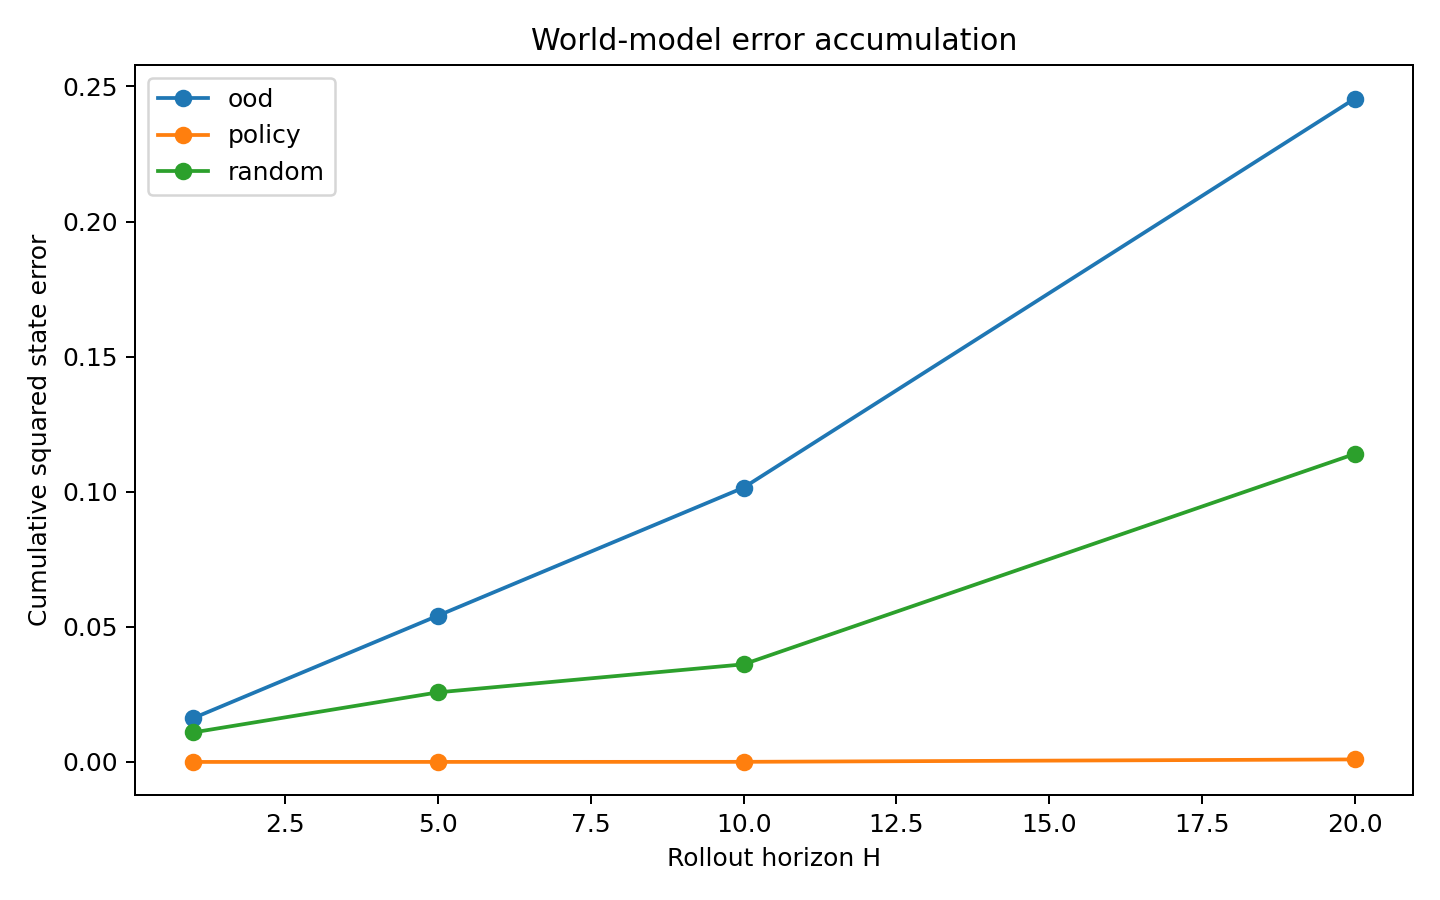
\includegraphics[width=0.66\linewidth]{../runs/world_model_eval/rollout_error.png}
\caption{Cumulative rollout error stays flat on-distribution and diverges off-distribution, compounding
with horizon --- the toy analogue of long-horizon hallucination.}
\end{figure}}{}

\subsection{Phase 3 --- Policy refinement inside the world model}
A vectorized imagined environment applies the exact reward, uses the ensemble mean as the next state, and
the ensemble variance as $u_t$. A real PPO checkpoint warm-starts the policy (RL post-training in
imagination). Four methods are compared:
\begin{itemize}[leftmargin=1.4em,itemsep=2pt]
  \item \textbf{Fixed $H{=}5$ / $H{=}20$}: fixed imagined-rollout length (longer $H$ = stronger credit
  assignment but more error accumulation).
  \item \textbf{Uncertainty termination}: cut the rollout when $u_t>\tau$ ($\tau=q_{95}$), an
  \emph{adaptive} horizon $H_t=\min\{H_{\max},\,\text{first }t:u_t>\tau\}$ --- the toy counterpart of
  WoVR's KIR error-depth control.
  \item \textbf{Weighted advantage}: down-weight uncertain transitions,
  $\tilde A_t=w_t\hat A_t$, $w_t=\max(0.02,\exp(-\beta\,u_t/\tau))$ --- confidence-weighted updates.
\end{itemize}

\subsection{Phase 4 --- The exploitation gap}
Because short imagined-segment returns are not comparable across horizons, every policy is evaluated from
\emph{matched} initial states for a common 200-step horizon in both worlds:
\begin{equation}
\Jmodel(\pi)=\tfrac1N\!\sum_i R^{(i)}_{\mathrm{model}},\quad
\Jreal(\pi)=\tfrac1N\!\sum_i R^{(i)}_{\mathrm{real}},\quad
\textbf{Exploitation Gap}=\Jmodel(\pi)-\Jreal(\pi).
\end{equation}
A positive gap means the policy looks better in imagination than in reality --- it is exploiting model
error. Two regimes are studied.

\paragraph{Regime A --- refine the in-distribution (near-optimal) policy.} Warm-starting from the same
policy that generated the model's data, the model is so faithful that model $\approx$ real everywhere
(gap $\approx0$ for $H{=}20$ and uncertainty termination). There is nothing to exploit and no headroom to
improve --- a degenerate regime.

\paragraph{Regime B --- refine an off-distribution (sub-optimal) policy.} Warm-starting instead from a
deliberately sub-optimal checkpoint ($\approx{-}570$), 500k imagined steps, 3 seeds, against the
\emph{same} expert-trained model, the exploitation gap appears (Table~\ref{tab:gap}) and is largest at
$H{=}20$ --- consistent with more error accumulation over longer rollouts.

\begin{table}[h]
\centering
\caption{Phase 4, Regime B: 200-step model-vs-real comparison (mean $\pm$ std over 3 seeds).}
\label{tab:gap}
\begin{tabular}{lccc}
\toprule
Method & Real return & Exploitation gap & Mean horizon\\
\midrule
mid init (baseline)      & $-576$ & $-3$ & ---\\
Fixed $H{=}5$            & $-792\pm249$ & $+20\pm22$ & $5.0$\\
Fixed $H{=}20$           & $-754\pm105$ & $\mathbf{+28\pm21}$ & $20.0$\\
Uncertainty termination  & $-1473\pm24$ & $+9\pm26$ & $\mathbf{4.3}$\\
Weighted advantage $H{=}20$ & $-1462\pm4$ & $-13\pm1$ & $20.0$\\
\bottomrule
\end{tabular}
\end{table}

\IfFileExists{../runs/comparison_seeds/exploitation_gap_seeds.png}{%
\begin{figure}[h]\centering
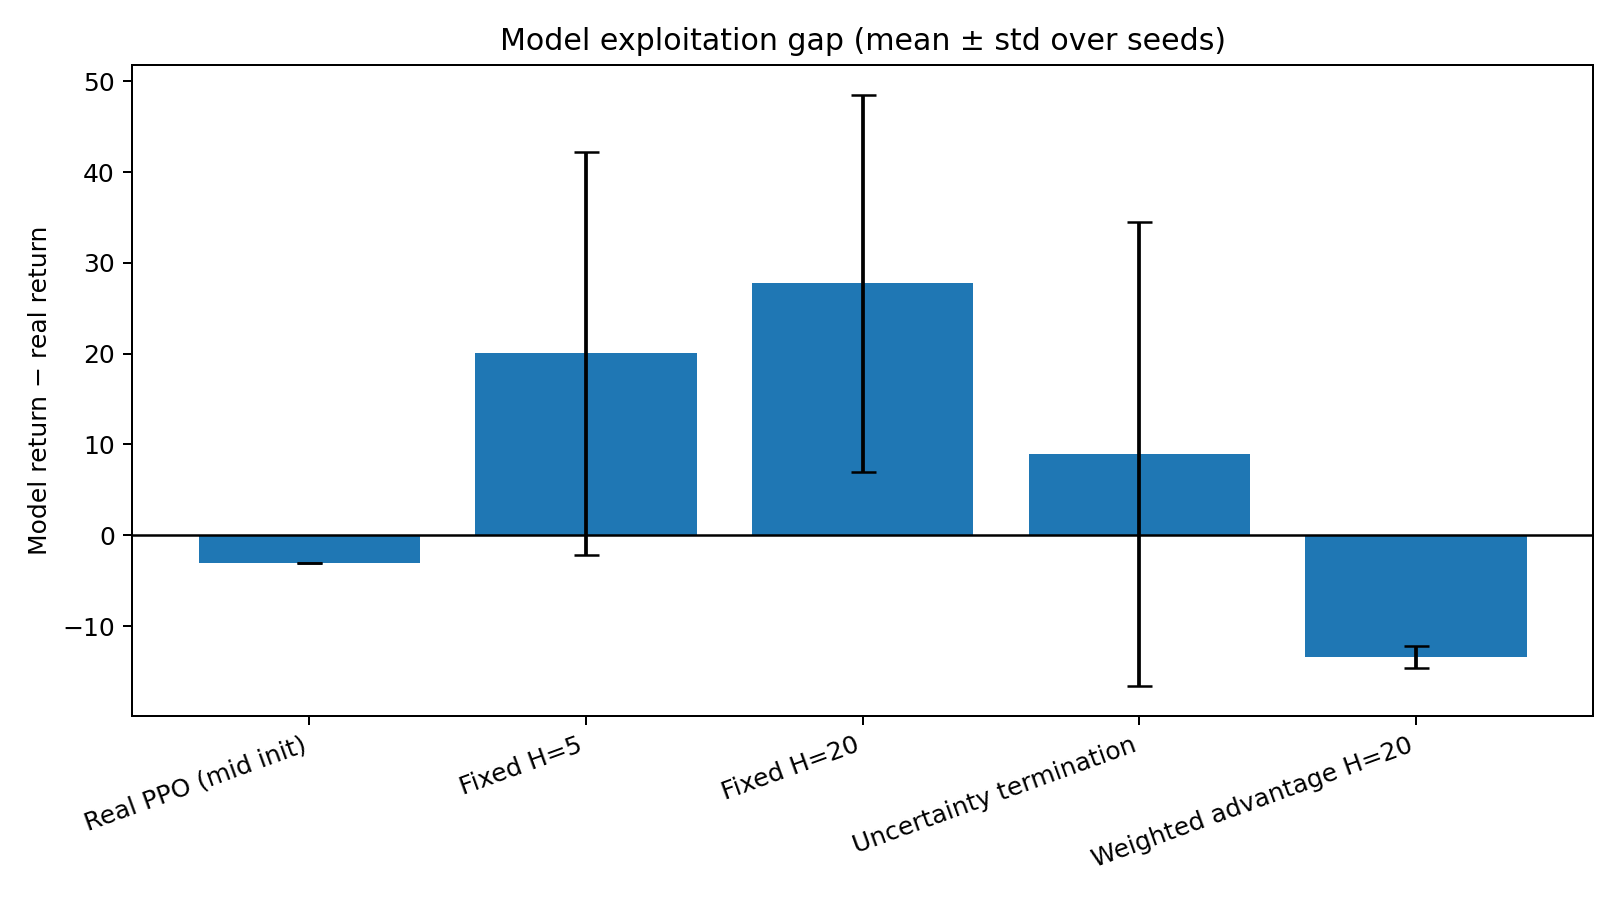
\includegraphics[width=0.72\linewidth]{../runs/comparison_seeds/exploitation_gap_seeds.png}
\caption{Exploitation gap across seeds (Regime B). The gap is largest for fixed long-horizon rollouts.}
\end{figure}}{}

\subsection{Key finding: two regimes, and why the safeguards did not transfer}
Combining the regimes gives a sharper statement than either alone. (1) In-distribution refinement is safe
but uninformative. (2) Off-distribution refinement produces a genuine, horizon-growing exploitation gap
under fixed rollouts --- \emph{and} the uncertainty machinery, calibrated on the narrow expert
distribution ($q_{95}=6.6\times10^{-6}$), does not transfer: the sub-optimal policy induces uncertainty
$\sim10^{-5}$ almost everywhere, so termination fires immediately (adaptive horizon collapses $20\to4.3$),
starving credit assignment, while weighted advantages down-weight nearly every transition. Both
``safeguards'' therefore \emph{hurt} real return here.

The lesson is not ``these methods fail,'' but the more precise and useful one: \textbf{a static world
model supports reliable policy improvement only within its training distribution, and uncertainty
thresholds must be calibrated on the distribution the policy actually visits.} This is exactly
long-horizon error accumulation and policy-induced distribution shift made measurable on a controllable
toy --- and it independently points at the two papers' remedies.

\begin{table}[h]
\centering
\caption{Mechanism-level correspondence between this reproduction and the two papers.}
\label{tab:map}
\begin{tabular}{p{4.6cm}p{5.0cm}p{4.6cm}}
\toprule
Reproduction finding & World4RL & WoVR\\
\midrule
Off-distribution refinement collapses; model needs coverage of visited states &
Train the world model on expert $\cup$ policy $\cup$ \emph{random} rollouts; broader action-space
coverage & Distribution shift as a core failure mode\\
\addlinespace
Fixed long horizon $\Rightarrow$ larger exploitation gap &
--- & KIR shortens effective error depth\\
\addlinespace
Narrow-distribution uncertainty thresholds stop transferring after policy shift &
Controlled exploration (std clipping) keeps the policy in-support &
PACE co-evolves the model with the evolving policy\\
\bottomrule
\end{tabular}
\end{table}

\subsection{Limitations and future work}
The decisive next step is to train the ensemble on \emph{broad} replay data (e.g.\ policy $\cup$ random)
and recalibrate uncertainty there --- the toy analogue of World4RL's random rollouts and WoVR's PACE ---
which is expected to let the uncertainty-aware methods recover real return and shrink the gap. Iterative
data collection (MBPO-style) is the principled cure for policy-induced shift; Regime A should also be
seeded before drawing quantitative conclusions. Everything here is a 3-D state space, but the mechanisms
(delta dynamics, ensemble uncertainty, imagined refinement, exploitation-gap measurement) transfer to
higher-dimensional and pixel/latent world models.

% ===========================================================================
\section*{Note on scope}
\addcontentsline{toc}{section}{Note on scope}
This is a focused, from-scratch reproduction and mechanism study built to understand how policy
optimization stays reliable under an imperfect learned model. It reproduces state-space dynamics-model
MBRL, not a generative or video world model, and reports results --- including a safeguard that fails to
transfer off-distribution --- as measured. Code and figures:
\url{https://github.com/TanhJK728/world-model-rl}.

% ===========================================================================
\begin{thebibliography}{9}
\bibitem{world4rl} Z.\ Jiang, K.\ Liu, Y.\ Qin, S.\ Tian, Y.\ Zheng, M.\ Zhou, C.\ Yu, H.\ Li,
D.\ Zhao. \emph{World4RL: Diffusion World Models for Policy Refinement with Reinforcement Learning for
Robotic Manipulation.} arXiv:2509.19080, 2025.
\bibitem{wovr} Z.\ Jiang, S.\ Zhou, et al. \emph{WoVR: World Models as Reliable Simulators for
Post-Training VLA Policies with RL.} arXiv:2602.13977, 2026.
\bibitem{ppo} J.\ Schulman, F.\ Wolski, P.\ Dhariwal, A.\ Radford, O.\ Klimov. \emph{Proximal Policy
Optimization Algorithms.} arXiv:1707.06347, 2017.
\bibitem{gae} J.\ Schulman, P.\ Moritz, S.\ Levine, M.\ Jordan, P.\ Abbeel. \emph{High-Dimensional
Continuous Control Using Generalized Advantage Estimation.} ICLR, 2016.
\bibitem{pets} K.\ Chua, R.\ Calandra, R.\ McAllister, S.\ Levine. \emph{Deep Reinforcement Learning in a
Handful of Trials using Probabilistic Dynamics Models (PETS).} NeurIPS, 2018.
\bibitem{mbpo} M.\ Janner, J.\ Fu, M.\ Zhang, S.\ Levine. \emph{When to Trust Your Model: Model-Based
Policy Optimization (MBPO).} NeurIPS, 2019.
\bibitem{dreamer} D.\ Hafner, J.\ Pasukonis, J.\ Ba, T.\ Lillicrap. \emph{Mastering Diverse Control Tasks
through World Models (DreamerV3).} Nature, 2025.
\bibitem{grpo} Z.\ Shao et al. \emph{DeepSeekMath: Pushing the Limits of Mathematical Reasoning (GRPO).}
arXiv:2402.03300, 2024.
\bibitem{edm} T.\ Karras, M.\ Aittala, S.\ Laine, S.\ Aila. \emph{Elucidating the Design Space of
Diffusion-Based Generative Models (EDM).} NeurIPS, 2022.
\end{thebibliography}

\end{document}
